% ============================================================
%  §1  Manipulating Inequalities and the Logic of Bounding
%  volume-iii/analysis/real-analysis/notes/proof-techniques/
%  01-inequalities-bounding.tex
% ============================================================

\section{Manipulating Inequalities and the Logic of Bounding}
\label{sec:inequality-bounding}

\begin{tcolorbox}[colback=gray!6, colframe=gray!40, arc=2pt,
  left=6pt, right=6pt, top=4pt, bottom=4pt,
  title={\small\textbf{Inequality Toolkit — Quick Reference}},
  fonttitle=\small\bfseries]
\small
\begin{tabular}{l l l}
\toprule
\textbf{Tool} & \textbf{Statement} & \textbf{Typical use} \\
\midrule
Triangle inequality
  & $|a+b|\leq|a|+|b|$
  & Split a distance at an intermediate point \\[3pt]
Distance form
  & $|a-b|\leq|a-c|+|c-b|$
  & Introduce pivot $c$ to separate two estimates \\[3pt]
Reverse triangle ineq.
  & $\bigl\lvert|a|-|b|\bigr\rvert\leq|a-b|$
  & Bound magnitudes using closeness \\[3pt]
Absolute value interval
  & $|x|\leq y\;\Longleftrightarrow\;{-y}\leq x\leq y$
  & Convert $|\cdot|$ bound to two-sided inequality \\[3pt]
Boundedness replacement
  & $|b_n|\leq M$ (constant): replace $|b_n|$ by $M$
  & Eliminate variable factors in products \\[3pt]
$\varepsilon$-budget split
  & $|A|<\tfrac{\varepsilon}{2}$ and $|B|<\tfrac{\varepsilon}{2}$
    $\Rightarrow|A+B|<\varepsilon$
  & Combine two independent estimates \\[3pt]
$+1$ trick
  & Replace $|L|$ by $|L|+1$ in denominators
  & Avoid division by zero when $L$ may vanish \\
\bottomrule
\end{tabular}
\end{tcolorbox}

% ── §1.1: Asymmetry ──────────────────────────────────────────
\subsection{The Fundamental Asymmetry Between Equality and Inequality}
\label{subsec:ineq-asymmetry}

Equality is bilateral: $a=b$ licenses substitution in either direction and
carries no information about magnitude. An inequality is directional:
$a\leq b$ locates $a$ relative to $b$ on the line, says nothing about the
gap, and does not support backwards substitution.

This asymmetry is the source of a strategic shift. In an equality argument
the goal is to show that two expressions are the same object. In a bounding
argument the goal is to show that one expression is \emph{controlled} by
another. Control is inherently one-sided: a ceiling above $|f(x)|$ is useful
regardless of how far below it $|f(x)|$ actually falls.

\begin{remark}[Consequence for proof strategy]
The question in analysis is rarely ``what is $|a_n-L|$?'' It is ``is
$|a_n-L|$ smaller than $\varepsilon$?'' A valid crude bound that answers the
second question is more useful than an exact answer to the first. Deliberate
over-estimation — absent from algebra — is a required habit.
\end{remark}

\begin{remark}[Common error]
Treating an inequality as if it were an equality by reversing direction.
Given $a\leq b$, negation gives $-a\geq -b$, not $-a\leq -b$. Multiplication
by a negative constant reverses direction. Failing to track sign changes
when multiplying or negating is the most frequent algebraic error in
$\varepsilon$-$\delta$ computations.
\end{remark}

% ── §1.2: Basic rules ────────────────────────────────────────
\subsection{The Basic Rules of Inequality Arithmetic}
\label{subsec:ineq-rules}

\begin{proposition}[Order arithmetic]
\label{prop:order-arithmetic}
Let $a,b,c,d\in\mathbb{R}$.
\begin{enumerate}[label=(\roman*)]
  \item If $a\leq b$ and $c\leq d$, then $a+c\leq b+d$.
  \item If $a\leq b$ and $c>0$, then $ac\leq bc$.
  \item If $a\leq b$ and $c<0$, then $ac\geq bc$.
  \item $|x|\leq y$ (with $y\geq 0$) if and only if $-y\leq x\leq y$.
\end{enumerate}
\end{proposition}

\begin{remark*}[Flash]
\FlashQ{State the order arithmetic properties of $\mathbb{R}$.}
\FlashA{(i) $a\le b,c\le d\Rightarrow a+c\le b+d$; (ii) $a\le b,c>0\Rightarrow ac\le bc$; (iii) $a\le b,c<0\Rightarrow ac\ge bc$.}
\FlashHint{Multiplication by a negative flips the inequality.}
\end{remark*}


\begin{remark}[Fully quantified form]
(i) $\forall a,b,c,d\in\mathbb{R},\;(a\leq b)\land(c\leq d)
    \Rightarrow a+c\leq b+d$. \quad
(iv) $\forall x\in\mathbb{R},\;\forall y\geq 0,\;
    |x|\leq y\;\Leftrightarrow\;-y\leq x\leq y$.
\end{remark}

\begin{remark}[Inequalities add but do not subtract]
Rule (i) licenses adding inequalities in the same direction. There is no
subtraction rule: $a\leq b$ and $c\leq d$ yields no conclusion about
$a-c$ versus $b-d$ in general. The direction of $a-c$ versus $b-d$ depends
on the relative sizes of $(b-a)$ and $(d-c)$, which are not controlled.
\end{remark}

\begin{remark}[Consequence for absolute values]
Rule (iv) is the bridge between $|\cdot|$ bounds and two-sided linear
inequalities. It is invoked silently every time an $\varepsilon$-$N$ argument
converts $|a_n-L|<\varepsilon$ into positional information about $a_n$.
\end{remark}

% figure-absolute-value-interval.tex — inline, no float wrapper.
% Requires \usepackage{caption} in main.tex for \captionof.

\begin{center}
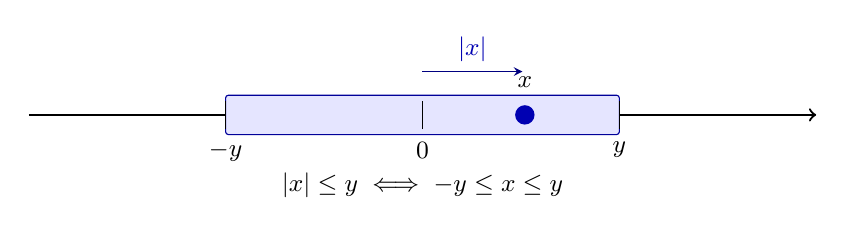
\begin{tikzpicture}[
  lbl/.style={font=\small},
  tick/.style={thin},
  arr/.style={->, >=stealth, thin}
]
\draw[thick, ->] (-0.5, 0) -- (9.5, 0);
\draw[fill=blue!10!white, draw=blue!60!black, rounded corners=1pt]
  (2.0, -0.25) rectangle (7.0, 0.25);
\draw[tick] (2.0, -0.18) -- (2.0, 0.18);
\draw[tick] (4.5, -0.18) -- (4.5, 0.18);
\draw[tick] (7.0, -0.18) -- (7.0, 0.18);
\node[lbl, below] at (2.0, -0.22) {$-y$};
\node[lbl, below] at (4.5, -0.22) {$0$};
\node[lbl, below] at (7.0, -0.22) {$y$};
\fill[blue!70!black] (5.8, 0) circle (3.5pt);
\node[lbl, above] at (5.8, 0.22) {$x$};
\draw[->, >=stealth, thin, draw=blue!50!black]
  (4.5, 0.55) -- (5.77, 0.55)
  node[midway, above, font=\small, text=blue!70!black] {$|x|$};
\node[lbl] at (4.5, -0.9)
  {$|x| \leq y \;\Longleftrightarrow\; -y \leq x \leq y$};
\end{tikzpicture}
\end{center}
\captionof{figure}{%
  The absolute value characterisation as a symmetric interval. The shaded
  region is $[-y, y]$; the point $x$ lies inside with $|x| \leq y$.
  The equivalence $|x| \leq y \Leftrightarrow -y \leq x \leq y$
  (Proposition~\ref{prop:order-arithmetic}(iv)) converts an absolute value
  bound into a two-sided linear constraint.%
}
\label{fig:absolute-value-interval}
\medskip


% ── §1.3: Triangle inequality ────────────────────────────────
\subsection{The Triangle Inequality and the Pivot Move}
\label{subsec:triangle-ineq}

\begin{tcolorbox}[colback=thmbox, colframe=thmborder, arc=2pt,
  left=6pt, right=6pt, top=4pt, bottom=4pt,
  title={\small\textbf{Theorem (Triangle Inequality)}},
  fonttitle=\small\bfseries]
\label{thm:triangle-inequality}
For all $a,b\in\mathbb{R}$, $\;|a+b|\leq|a|+|b|$. Equivalently, for all
$a,b,c\in\mathbb{R}$, $\;|a-b|\leq|a-c|+|c-b|$.
\end{tcolorbox}

\begin{remark}[Fully quantified form]
$\forall a,b\in\mathbb{R},\;|a+b|\leq|a|+|b|$.
\end{remark}

\begin{remark}[The pivot move]
The distance form $|a-b|\leq|a-c|+|c-b|$ is the operative version in
analysis. The element $c$ is a \emph{pivot}: an intermediate point that
decomposes a hard distance into two pieces, each controllable by hypothesis.
In the proof that $a_n+b_n\to L+M$, the pivot $c=L+b_n$ gives
\[
  |(a_n+b_n)-(L+M)|
  =|(a_n-L)+(b_n-M)|
  \leq|a_n-L|+|b_n-M|,
\]
and the two pieces are controlled by the individual convergences.
\end{remark}

\begin{remark}[Reverse triangle inequality]
\label{rem:reverse-tri}
$\bigl\lvert|a|-|b|\bigr\rvert\leq|a-b|$. Proof: apply the standard
inequality to $a=(a-b)+b$ to get $|a|-|b|\leq|a-b|$; symmetry gives the
other side. Consequence: $|\cdot|:\mathbb{R}\to\mathbb{R}$ is Lipschitz
with constant $1$, so closeness of inputs implies closeness of magnitudes.
\end{remark}

\begin{remark}[Common error]
Writing $|a|+|b|\leq|a+b|$. The triangle inequality always produces an
\emph{upper} bound on a sum, never a lower bound. The reverse
($|1|+|-1|=2>|1+(-1)|=0$) is a one-line counterexample.
\end{remark}

% figure-triangle-inequality-pivot.tex — inline, no float wrapper.

\begin{center}
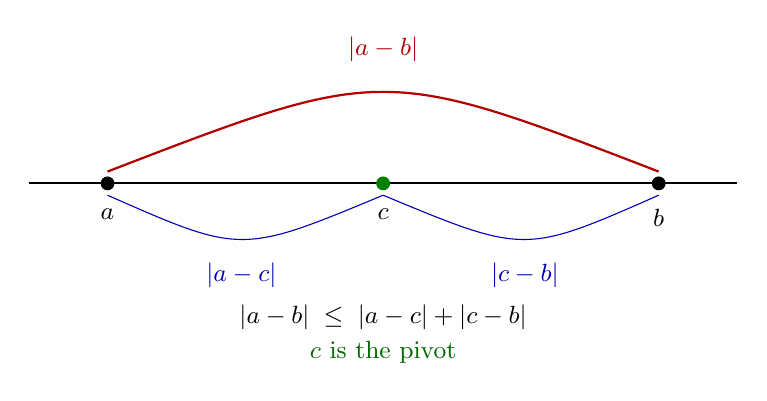
\begin{tikzpicture}[
  dot/.style={circle, fill, inner sep=0pt, minimum size=5pt},
  lbl/.style={font=\small}
]
\draw[thick] (0.5, 0) -- (9.5, 0);
\node[dot] (a) at (1.5, 0) {};
\node[dot, fill=green!50!black] (c) at (5.0, 0) {};
\node[dot] (b) at (8.5, 0) {};
\node[lbl, below] at (1.5, -0.2) {$a$};
\node[lbl, below] at (5.0, -0.2) {$c$};
\node[lbl, below] at (8.5, -0.2) {$b$};
\draw[red!70!black, thick]
  (1.5, 0.15) .. controls (5.0, 1.5) .. (8.5, 0.15);
\node[lbl, above, text=red!70!black] at (5.0, 1.42) {$|a-b|$};
\draw[blue!70!black]
  (1.5, -0.15) .. controls (3.2, -0.9) .. (5.0, -0.15);
\node[lbl, below, text=blue!70!black] at (3.2, -0.88) {$|a-c|$};
\draw[blue!70!black]
  (5.0, -0.15) .. controls (6.8, -0.9) .. (8.5, -0.15);
\node[lbl, below, text=blue!70!black] at (6.8, -0.88) {$|c-b|$};
\node[lbl] at (5.0, -1.7) {$|a-b| \;\leq\; |a-c| + |c-b|$};
\node[lbl, text=green!40!black] at (5.0, -2.15) {$c$ is the pivot};
\end{tikzpicture}
\end{center}
\captionof{figure}{%
  The triangle inequality in distance form. The direct distance $|a-b|$
  (red) is bounded above by the sum of indirect distances $|a-c|$ and
  $|c-b|$ (blue) through pivot $c$. In analysis, $c$ is chosen to split
  $|a-b|$ into two pieces each controlled by a separate hypothesis.%
}
\label{fig:triangle-inequality-pivot}
\medskip


% ── §1.4: Bounding is not solving ────────────────────────────
\subsection{Bounding Is Not Solving}
\label{subsec:bounding-not-solving}

In algebra, a computation terminates when the exact value is found. In
analysis, a bounding argument terminates when the expression is shown to
fall within an acceptable range. These are structurally different goals.

\begin{remark}[Deliberate crudeness is valid]
To bound $|x^2-9x+1|$ on $[-1,5]$:
\[
  |x^2-9x+1|\leq|x|^2+9|x|+1\leq 25+45+1=71.
\]
The actual supremum is far smaller than $71$. That is irrelevant. The bound
is valid, explicit, and was obtained cheaply. The test for a bound is not
``is this sharp?'' but ``is this true and sufficient for the argument's
purpose?''
\end{remark}

\begin{remark}[Consequence for proof reading]
A reader who checks that each inequality is valid can trust the conclusion
without caring whether the bounds are optimal. Optimality is irrelevant to
logical correctness.
\end{remark}

% ── §1.5: ε-budget split ─────────────────────────────────────
\subsection{The $\varepsilon$-Budget Split}
\label{subsec:budget-split}

The prototype of all two-piece bounding arguments:
\[
  |A+B|\leq|A|+|B|<\frac{\varepsilon}{2}+\frac{\varepsilon}{2}=\varepsilon.
\]
The total tolerance $\varepsilon$ is a budget allocated among the summands.
With $k$ summands, allocate $\varepsilon/k$ each; with summands of unequal
difficulty, split unevenly provided the shares sum to at most $\varepsilon$.

\begin{remark}[The four-step procedure]
\label{rem:four-step}
Standard structure of an $\varepsilon$-$N$ or $\varepsilon$-$\delta$ proof:
\begin{enumerate}
  \item Apply the triangle inequality: express $|f-L|$ as a sum
        $|A_1|+\cdots+|A_k|$.
  \item Assign budgets $\varepsilon_i>0$ with $\sum_i\varepsilon_i=\varepsilon$.
  \item For each piece, find $N_i$ (or $\delta_i$) so that
        $|A_i|<\varepsilon_i$ for all $n\geq N_i$ (or $|x-a|<\delta_i$).
  \item Set $N=\max_i N_i$ (or $\delta=\min_i\delta_i$) to enforce all
        constraints simultaneously.
\end{enumerate}
Step 4 reflects the logical structure of the conclusion: all conditions must
hold at once, so the threshold is the most restrictive one.
\end{remark}

\begin{remark}[Common error]
Taking $N=N_1$ and ignoring $N_2$. For $n\geq N_1$ the first piece is
controlled; the second is not. Both pieces must be within budget simultaneously,
which requires $n\geq\max\{N_1,N_2\}$.
\end{remark}

% figure-epsilon-budget-split.tex — inline, no float wrapper.

\begin{center}
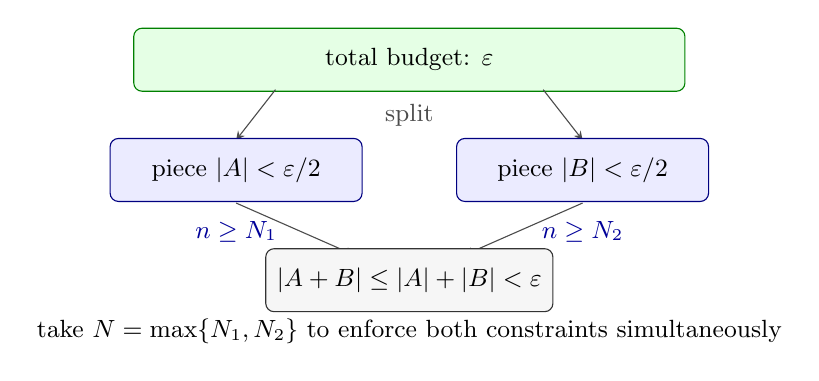
\begin{tikzpicture}[
  box/.style={draw, rounded corners=3pt, minimum width=3.2cm,
    minimum height=0.8cm, inner sep=4pt, font=\small},
  teal/.style={box, fill=green!10!white, draw=green!50!black},
  purp/.style={box, fill=blue!8!white, draw=blue!50!black},
  gray/.style={box, fill=gray!7!white, draw=gray!40!black},
  lbl/.style={font=\small},
  arr/.style={->, >=stealth, thin, gray!60!black}
]
\node[teal, minimum width=7.0cm] (tot) at (3.5, 3.2)
  {total budget: $\varepsilon$};
\draw[arr] (1.8, 2.82) -- (1.3, 2.18);
\draw[arr] (5.2, 2.82) -- (5.7, 2.18);
\node[lbl, gray!60!black] at (3.5, 2.5) {split};
\node[purp] (A) at (1.3, 1.8) {piece $|A| < \varepsilon/2$};
\node[lbl, below=3pt, text=blue!60!black] at (1.3, 1.38) {$n \geq N_1$};
\node[purp] (B) at (5.7, 1.8) {piece $|B| < \varepsilon/2$};
\node[lbl, below=3pt, text=blue!60!black] at (5.7, 1.38) {$n \geq N_2$};
\draw[arr] (1.3, 1.38) -- (2.8, 0.72);
\draw[arr] (5.7, 1.38) -- (4.2, 0.72);
\node[gray] (sum) at (3.5, 0.4)
  {$|A+B| \leq |A|+|B| < \varepsilon$};
\node[lbl] at (3.5, -0.25)
  {take $N = \max\{N_1, N_2\}$ to enforce both constraints simultaneously};
\end{tikzpicture}
\end{center}
\captionof{figure}{%
  The $\varepsilon$-budget split. The total tolerance $\varepsilon$ is
  distributed as shares $\varepsilon/2$ between two pieces. Each piece is
  controlled independently for $n \geq N_i$. Taking $N = \max\{N_1, N_2\}$
  enforces both bounds simultaneously, giving $|A+B| < \varepsilon$ for all
  $n \geq N$. With $k$ pieces, assign $\varepsilon/k$ each and take
  $N = \max_i N_i$.%
}
\label{fig:epsilon-budget-split}
\medskip


% ── §1.6: Boundedness replacement ────────────────────────────
\subsection{The Boundedness Replacement}
\label{subsec:boundedness-replacement}

\begin{proposition}[Convergent sequences are bounded]
\label{prop:convergent-bounded}
If $(b_n)\to b$, then there exists $M>0$ such that $|b_n|\leq M$ for all
$n\in\mathbb{N}$.
\end{proposition}

\begin{remark*}[Flash]
\FlashQ{State: convergent sequences are bounded.}
\FlashA{If $(b_n)\to b$ then $\exists M>0$ with $|b_n|\le M$ for all $n$.}
\FlashHint{Take $\varepsilon=1$: beyond $N$ all terms lie in $(b-1,b+1)$; finitely many terms before $N$ give a finite bound.}
\end{remark*}


\begin{remark}[Fully quantified form]
$\forall(b_n)\subset\mathbb{R},\;\lim_{n\to\infty}b_n=b
\;\Rightarrow\;
\exists M>0,\;\forall n\in\mathbb{N},\;|b_n|\leq M$.
\end{remark}

\begin{remark}[The replacement move]
Given $|b_n|\leq M$:
\[
  |b_n|\cdot|a_n-L|\leq M\cdot|a_n-L|.
\]
The variable factor is gone. Choose $N$ so that $|a_n-L|<\varepsilon/M$ for
$n\geq N$; the whole product is then less than $\varepsilon$. The constant $M$
need not be tight.
\end{remark}

\begin{remark}[Common error]
Choosing $|a_n-L|<\varepsilon/|b_n|$. This is circular: $N$ would depend on
$n$, since $|b_n|$ changes with $n$. The threshold $N$ must be a fixed
number, independent of $n$. Replacing $|b_n|$ by the constant $M$ breaks
the circularity.
\end{remark}

% ── §1.7: Work-backwards principle ───────────────────────────
\subsection{The Work-Backwards Principle}
\label{subsec:work-backwards}

$\varepsilon$-$N$ proofs are \emph{stated} forwards but \emph{discovered}
backwards. The proof asserts: ``Let $\varepsilon>0$. Choose
$N=\lceil C/\varepsilon\rceil$.'' The value $N$ was found by scratchwork:
``the expression simplifies to $C/n$; this is less than $\varepsilon$ when
$n>C/\varepsilon$; so set $N=\lceil C/\varepsilon\rceil$.''

The scratchwork is a private computation that produces the \emph{witness}.
The proof states the witness and verifies it, working forwards.

\medskip
\begin{tabular}{@{}ll@{}}
\textbf{Scratchwork (private):}
  & Work backwards from $|a_n-L|<\varepsilon$ to find what $N$ must satisfy.\\
\textbf{Proof (public):}
  & State $N$ explicitly. Verify $n\geq N\Rightarrow|a_n-L|<\varepsilon$.
\end{tabular}

\begin{remark}[Common error]
Allowing scratchwork to appear in the proof: ``we need $n>C/\varepsilon$, so
choose $n$ this large.'' The proof must assert a fixed $N$ and verify the
conclusion holds. A threshold stated as ``$n$ large enough'' is an incomplete
scratchwork note, not a proof.
\end{remark}

\begin{remark}[Connection to the geometric phase]
The work-backwards process is the analytic counterpart of the geometric phase
in limit proofs. The geometric phase identifies structure and chooses a pivot;
the backwards computation determines the explicit threshold. The proof states
both and verifies the chain forwards.
\end{remark}

% ── §1.8: Chaining inequalities ──────────────────────────────
\subsection{Chaining Inequalities}
\label{subsec:chaining}

A standard proof move builds a chain
$|f(x)|\leq A(x)\leq B\leq\varepsilon$,
where each step uses a different tool: the triangle inequality, a domain
bound, and the choice of $\delta$.

\begin{remark}[Replacing by a larger quantity]
A quantity on the right-hand side of $\leq$ may be freely replaced by
anything larger, since this only weakens the inequality. If
$|x|\leq|x-1|+1$ and $|x-1|<\delta$, then $|x|<\delta+1$. The replacement
of $|x-1|$ by $\delta$ is valid because $|x-1|$ appears on the right. The
same replacement on the \emph{left} would be invalid.
\end{remark}

\begin{remark}[Common error]
Including a step where the inequality points the wrong direction, or where
a step holds only generically rather than pointwise. A chain is only as
strong as its weakest link; every $\leq$ must be unconditionally valid.
\end{remark}

% ── §1.9: The +1 trick ───────────────────────────────────────
\subsection{The $+1$ Trick for Denominators}
\label{subsec:plus-one}

When $\varepsilon/|L|$ appears in an estimate and $L$ may be zero, replace
$|L|$ by $|L|+1\geq 1$:
\[
  \frac{\varepsilon}{|L|+1}\leq\varepsilon.
\]

\begin{remark}[Fully quantified form]
$\forall L\in\mathbb{R},\;|L|+1\geq 1>0$. Hence
$\varepsilon/(|L|+1)$ is well-defined and positive for all $\varepsilon>0$
and all $L\in\mathbb{R}$.
\end{remark}

\begin{remark}[Generalisation]
The $+1$ is an instance of a wider principle: any constant intended for a
denominator must be guaranteed strictly positive. If the constant is a
given quantity $C$ that might be zero, replace it by $C+1$. The choice of
$1$ is conventional; any fixed positive number serves the same purpose.
\end{remark}

\begin{remark}[Common error]
Using $|L|$ as a denominator without first verifying $L\neq 0$. The product
limit proof $a_nb_n\to LM$ is the canonical location for this error: the
bound $\varepsilon/(2|L|)$ fails when $L=0$, and the $L=0$ case requires
separate treatment or the use of $|L|+1$.
\end{remark}

% ── §1.10: Summary table ─────────────────────────────────────
\section*{Summary: The Bounding Mindset}

\medskip
\begin{tabular}{@{}ll@{}}
\toprule
\textbf{Algebra} & \textbf{Analysis} \\
\midrule
Find the exact value of $x$
  & Show $|x-L|<\varepsilon$ \\
Equality: both sides are the same object
  & Inequality: one side controls the other \\
Work backwards and forwards symmetrically
  & Discover witness backwards; verify forwards \\
Exact answer is the goal
  & Any valid bound is sufficient \\
Fractions must be simplified
  & Crude over-estimates are acceptable \\
Multiply both sides freely
  & Track sign changes; direction is load-bearing \\
\bottomrule
\end{tabular}
\medskip

\begin{remark}[The structure of a bounding proof]
A bounding proof is a \emph{chain of control}: inequalities connecting the
target expression to $\varepsilon$, where each link uses one of the toolkit
tools above. The proof is complete when the chain reaches $\varepsilon$.
Every link must be unconditionally valid; every variable factor must be
replaced by a constant before the chain can close.
\end{remark}